\documentclass[12pt]{article}
\title{EE445M Lab 4}
\author{Hershal Bhave (hb6279) and Eric Crosson (esc625)}
\date{Friday April 03, 2015}

\usepackage[in]{fullpage}
\usepackage{listings}
\usepackage{cleveref}
\usepackage[nosolutionfiles]{answers}
\usepackage{graphicx}
\usepackage{xcolor}
\usepackage{color}
\usepackage{enumerate}
\usepackage{pdfpages}
\usepackage{paracol}

\newenvironment{Ex}{\textbf{Problem}\vspace{.75em}\\}{}
\Newassociation{solution}{Soln}{Answers}
\pagebreak[3]
\newcommand{\Opentesthook}[2]{\Writetofile{#1}{\protect\section{#1: #2}}}
\renewcommand{\Solnlabel}[1]{\textbf{Solution}\quad}
\newcommand{\todo}{{\LARGE \emph{\color{red}TODO}}}

\newcommand{\dd}[1]{\:\mathrm{d}{#1}}
\newcommand{\ddt}[1]{\frac{\dd{}}{\dd{#1}}}
\newcommand{\dddt}[1]{\frac{\dd{}^2}{\dd{#1}^2}}

\definecolor{mygreen}{rgb}{0,0.6,0}
% \definecolor{mygreen}{rgb}{0.13,0.55,0.13}
\definecolor{mygray}{rgb}{0.5,0.5,0.5}
\definecolor{mymauve}{rgb}{0.58,0,0.82}

\lstset{
  backgroundcolor=\color{white},
  basicstyle=\scriptsize\ttfamily,
  breakatwhitespace=false,
  breaklines=true,
  captionpos=b,
  commentstyle=\color{mygreen},
  deletekeywords={...},
  escapeinside={\%*}{*)},
  extendedchars=true,
  frame=single,
  keywordstyle=\color{blue},
  % language=Octave,
  % numbers=left,
  % numbersep=5pt,
  % numberstyle=\tiny\color{mygray},
  rulecolor=\color{black},
  showspaces=false,
  showstringspaces=false,
  showtabs=false,
  % stepnumber=2,
  stringstyle=\color{mymauve},
  tabsize=2,
  title=\lstname,
  columns=fullflexible,
}

\begin{document}
\maketitle

\section{Objectives}
\begin{itemize}
\item Interface a microphone and record sounds
\item Design and implement an analog HPF, LPF and digital FIR filters
\item Build a spectrum analyzer
\item Write a real-time application that displays in both the time domain and the frequency domain
\end{itemize}

\section{Hardware Design}
Attached is a TI Webench Design Report of the analog low pass filter
used in this lab.
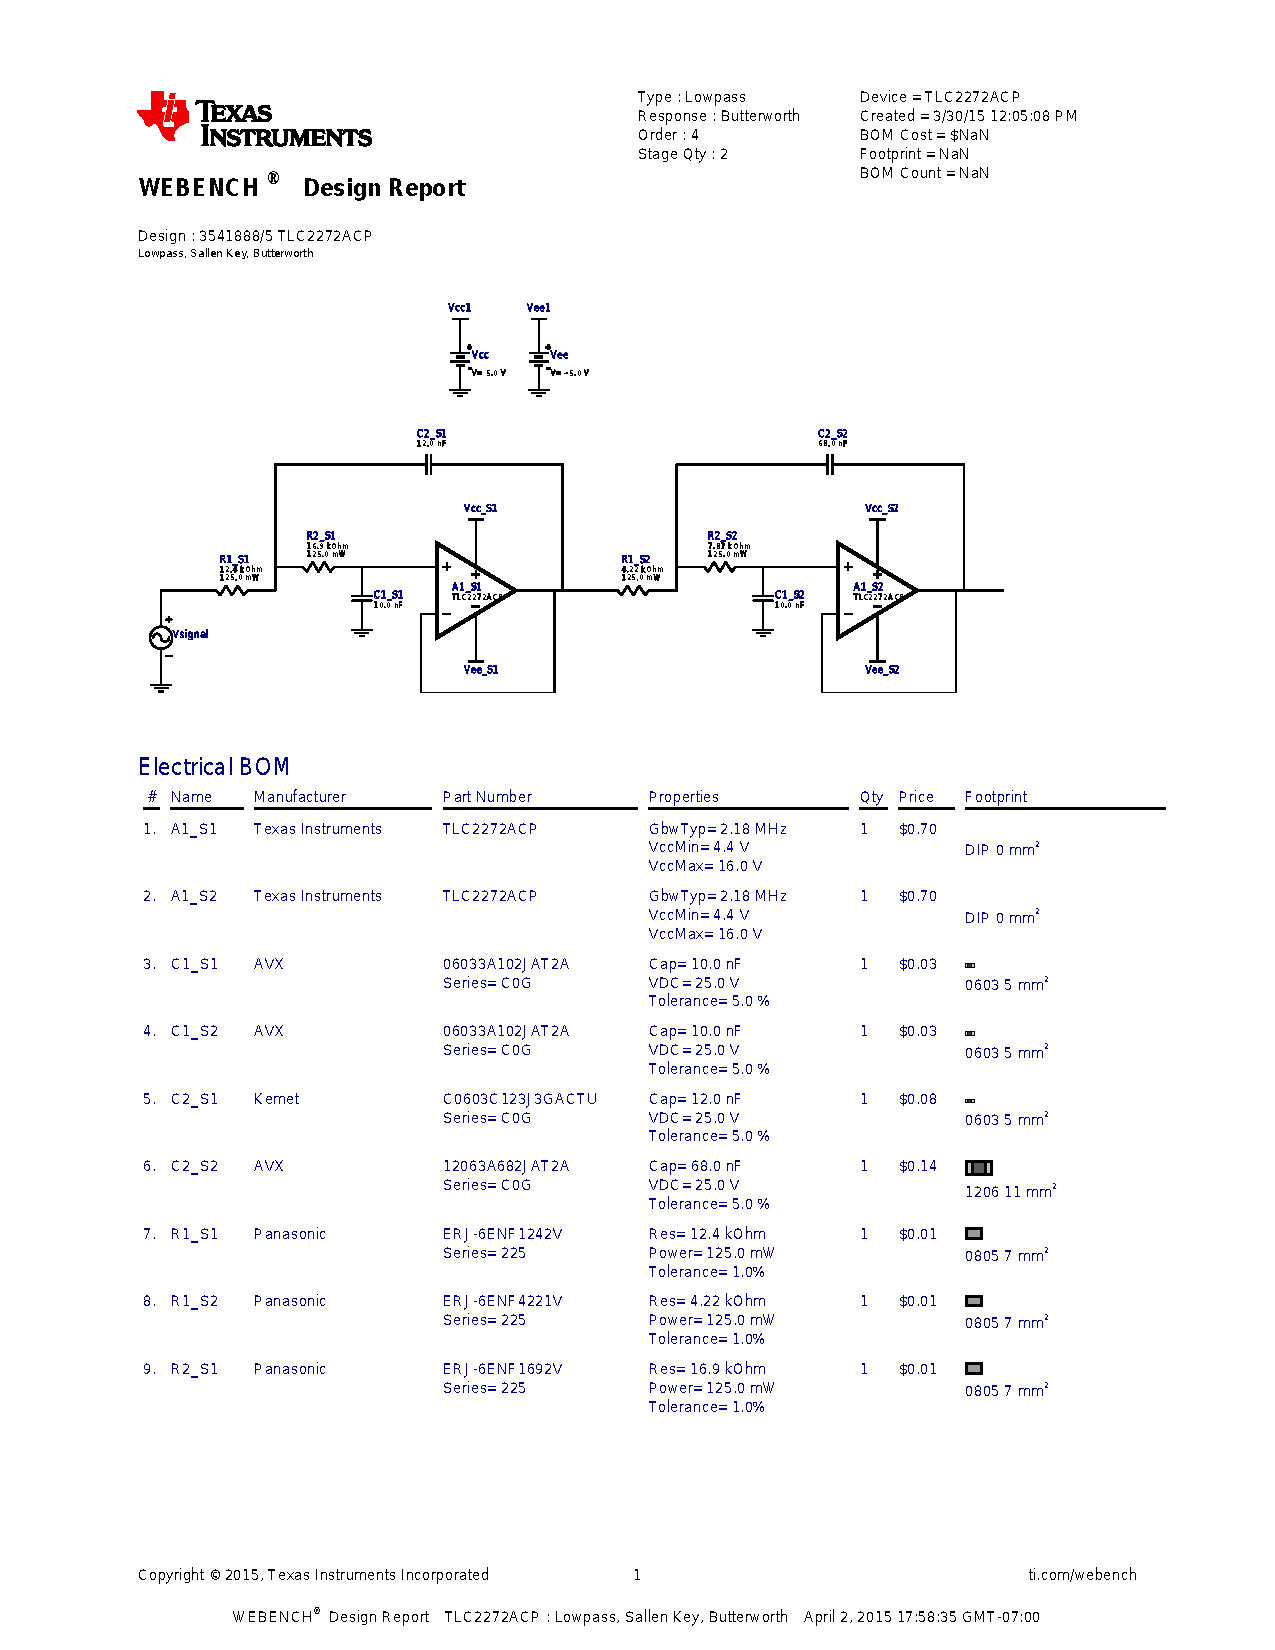
\includepdf[pages={1}]{./img/webench_analog_filter.pdf}

\section{Software Design}
Reference \cref{lst:lab4}. No extra magic is happening here - we have
distinct functions to handle the data manipulation (filtering, fft)
and discrete modes of operation. Semaphores guard shared resources and
timers dictate periodic tasks. Users may switch between
modes by entering commands through the shell via UART.

To facilitate debugging, we found it convenient to monitor operations
in the absence of periodic timer interrupts. Since SysTick is
responsible for the task switching, the only functionality periodic
timers were giving us related to ADC sampling at a specific rate. Each
trigger for ADC sampling started a lengthy data acquisition
process. To mitigate the need to work around these events while
debugging we introduce an adc simulator. The method
\verb|simulate_adc| iterates over a sine wave in memory and feeds the
sequential values into the FIFO that normally takes information from
the ADC. As such, normal program execution continues with
``simulated'' signals from a nonexistent signal generator.

Testing of each component (plot graphics, data acquisition, filter
accuracy, FFT) was by visual examination of output through the
LCD.

\section{Measurement Data}
\begin{enumerate}
\item Dynamic circuit performance \\
  Below are photographs of the LCD display during sampling of the a
  frequency of the indicated frequency from a signal generator. The
  axes are time vs. voltage.
  \begin{paracol}{2}
    \begin{figure}[h!]
      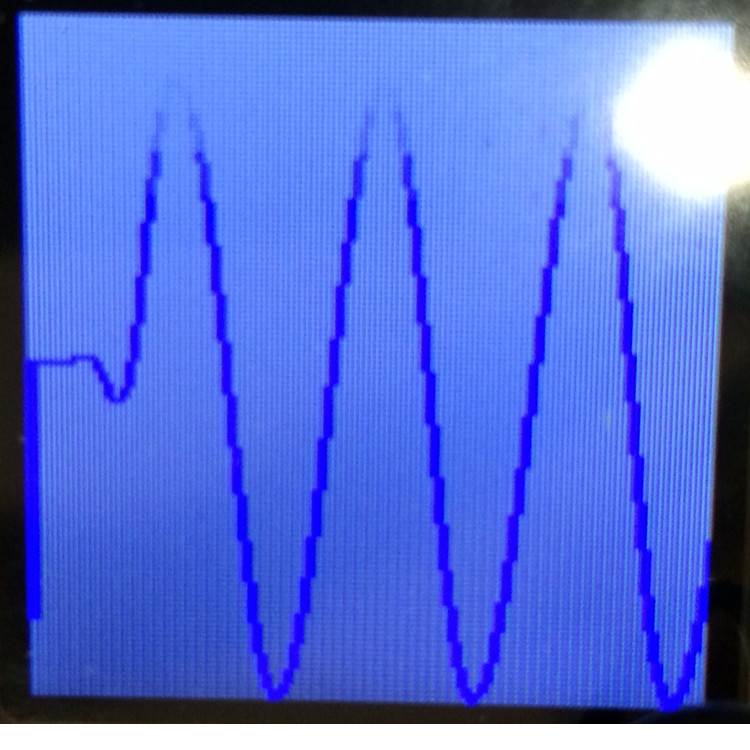
\includegraphics[width=0.375\textwidth]{./img/filtered_100Hz}
      \caption{\texttt{Filtered data 100 Hz plot}}
      \label{fig:filtered_100}
    \end{figure}
    \switchcolumn
    \begin{figure}[h!]
      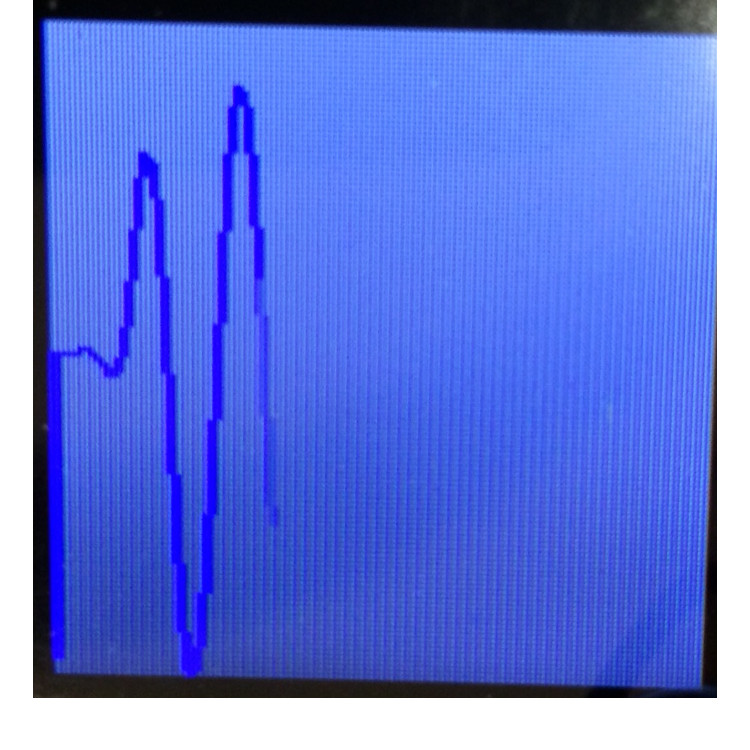
\includegraphics[width=0.375\textwidth]{./img/filtered_200Hz}
      \caption{\texttt{Filtered data 200 Hz plot}}
      \label{fig:filtered_200}
    \end{figure}
    \switchcolumn
    \begin{figure}[h!]
      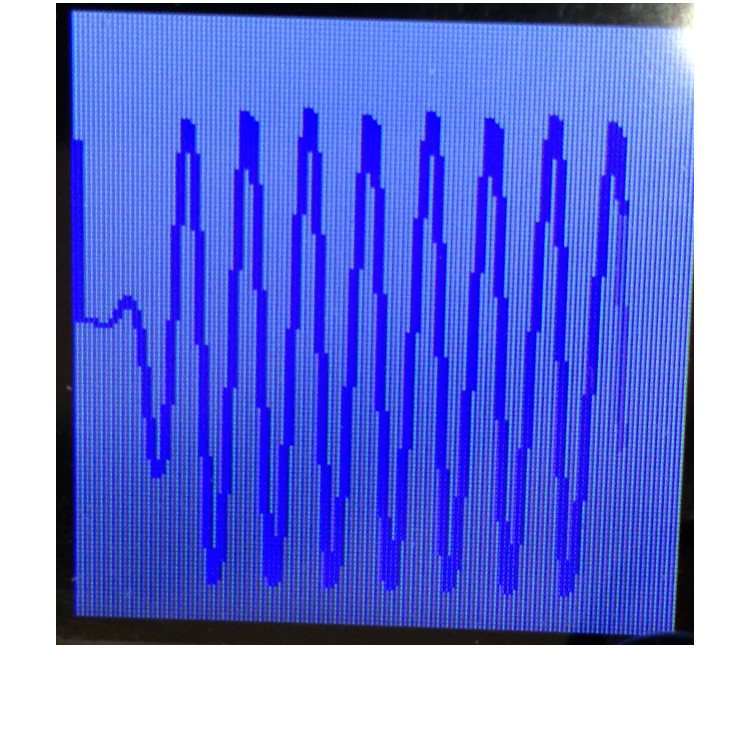
\includegraphics[width=0.375\textwidth]{./img/filtered_300Hz}
      \caption{\texttt{Filtered data 300 Hz plot}}
      \label{fig:filtered_300}
    \end{figure}
    \switchcolumn
    \begin{figure}[h!]
      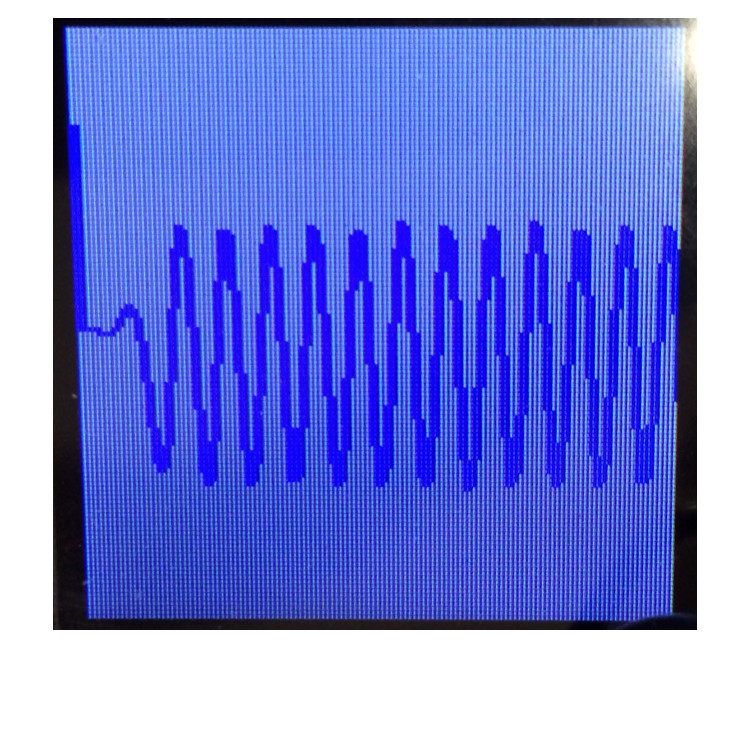
\includegraphics[width=0.375\textwidth]{./img/filtered_400Hz}
      \caption{\texttt{Filtered data 400 Hz plot}}
      \label{fig:filtered_400}
    \end{figure}
    \switchcolumn
    \begin{figure}[h!]
      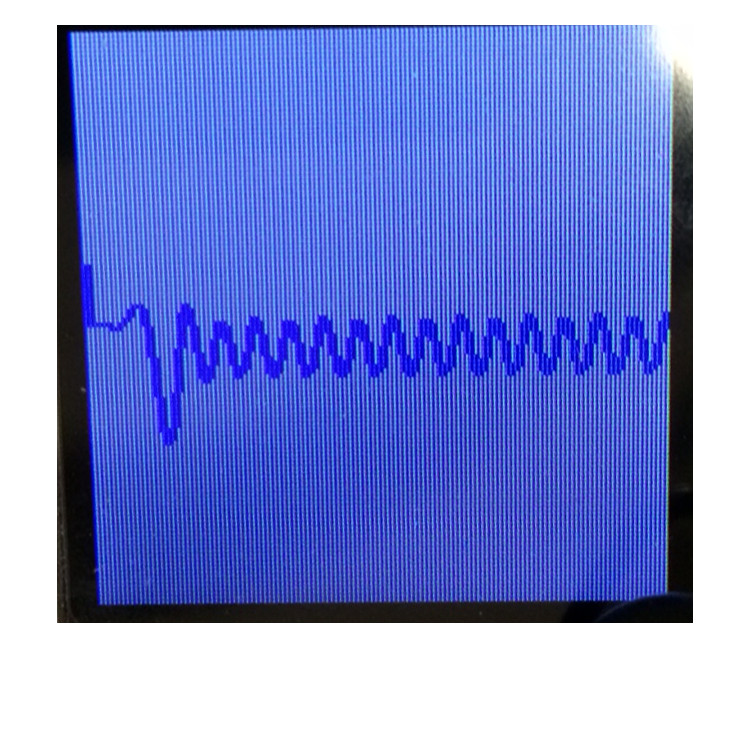
\includegraphics[width=0.375\textwidth]{./img/filtered_500Hz}
      \caption{\texttt{Filtered data 500 Hz plot}}
      \label{fig:filtered_500}
    \end{figure}
    \switchcolumn
    \begin{figure}[h!]
      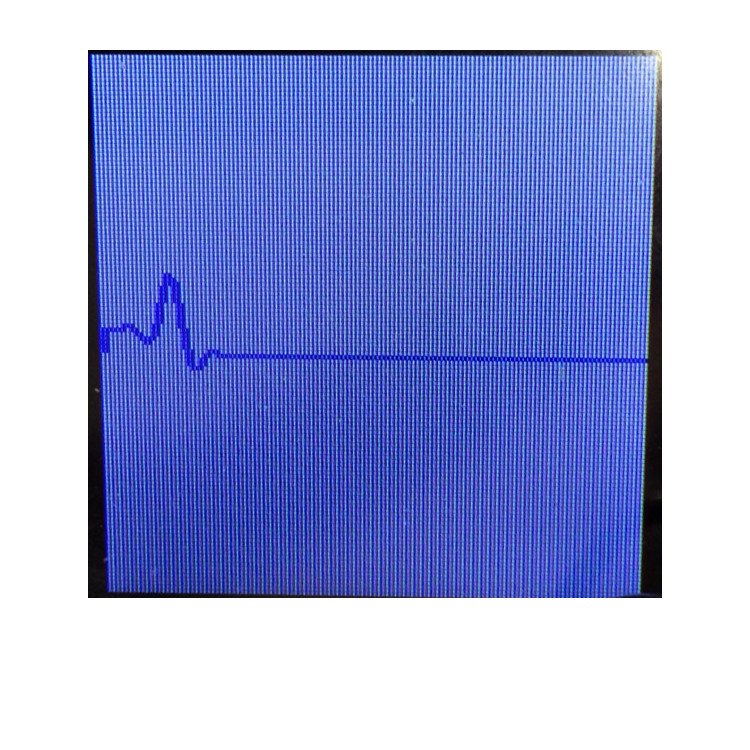
\includegraphics[width=0.375\textwidth]{./img/filtered_600Hz}
      \caption{\texttt{Filtered data 600 Hz plot}}
      \label{fig:filtered_600}
    \end{figure}
    \switchcolumn
    \begin{figure}[h!]
      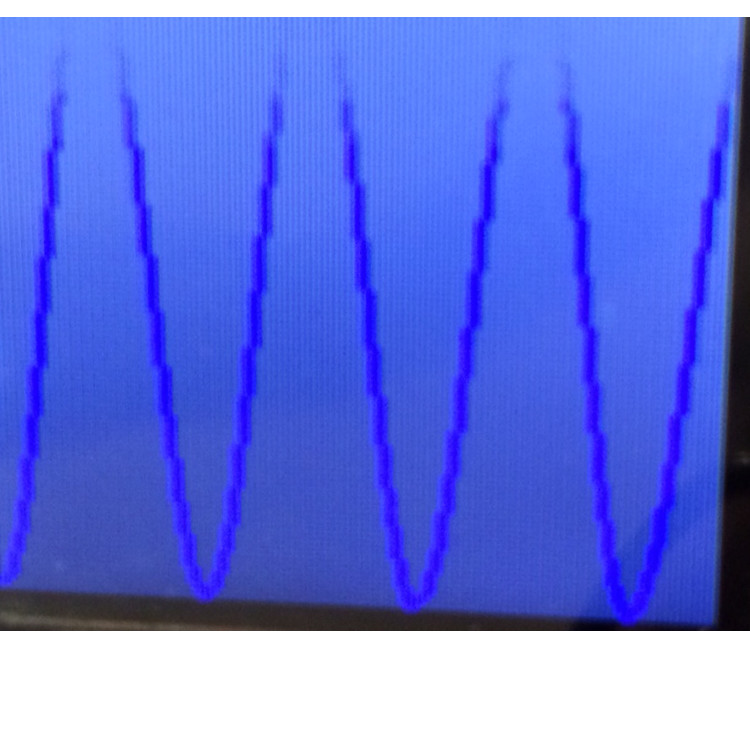
\includegraphics[width=0.375\textwidth]{./img/raw_100Hz}
      \caption{\texttt{Raw data 100 Hz plot}}
      \label{fig:raw_100}
    \end{figure}
    \switchcolumn
    \begin{figure}[h!]
      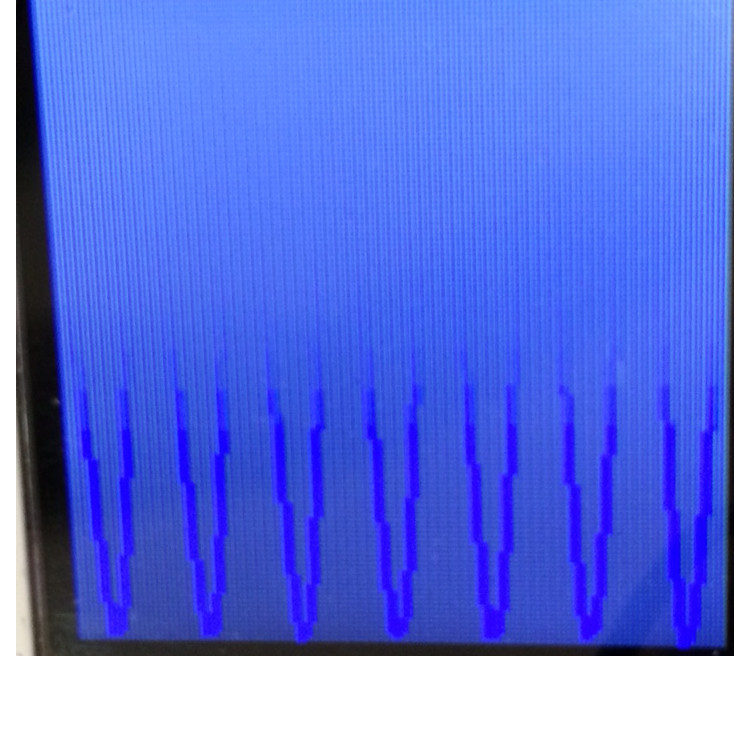
\includegraphics[width=0.375\textwidth]{./img/raw_200Hz}
      \caption{\texttt{Raw data 200 Hz plot}}
      \label{fig:raw_200}
    \end{figure}
    \switchcolumn
    \begin{figure}[h!]
      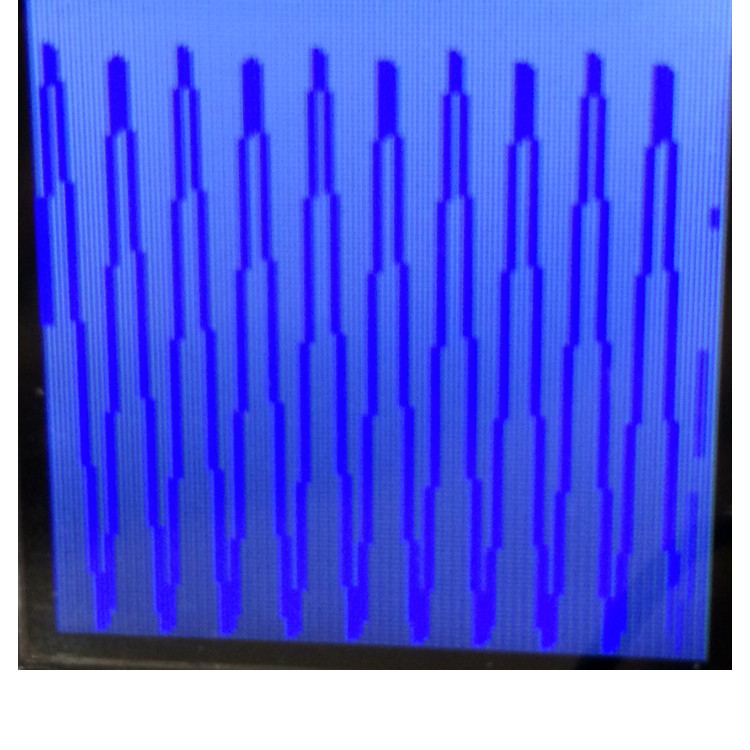
\includegraphics[width=0.375\textwidth]{./img/raw_300Hz}
      \caption{\texttt{Raw data 300 Hz plot}}
      \label{fig:raw_300}
    \end{figure}
    \switchcolumn
    \begin{figure}[h!]
      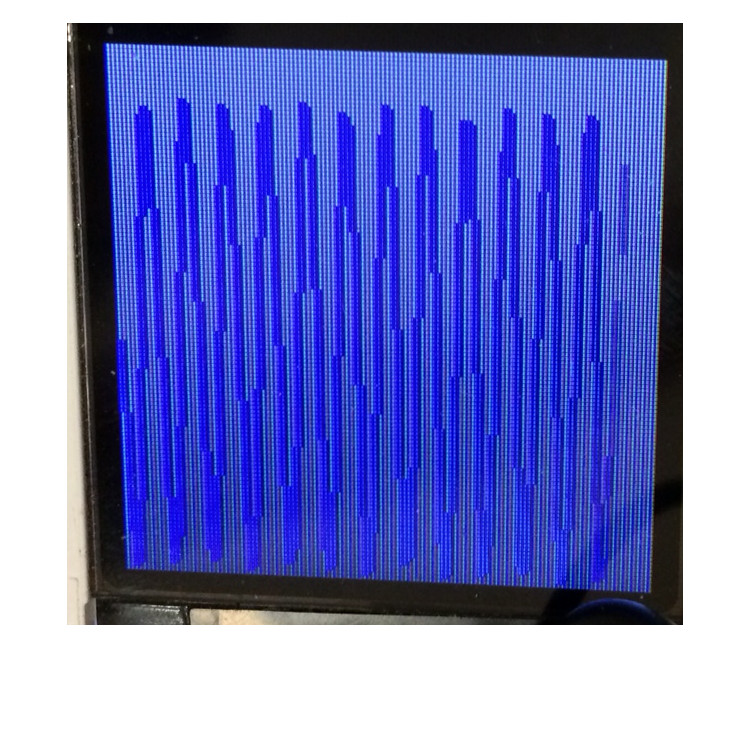
\includegraphics[width=0.375\textwidth]{./img/raw_400Hz}
      \caption{\texttt{Raw data 400 Hz plot}}
      \label{fig:raw_400}
    \end{figure}
    \switchcolumn
    \begin{figure}[h!]
      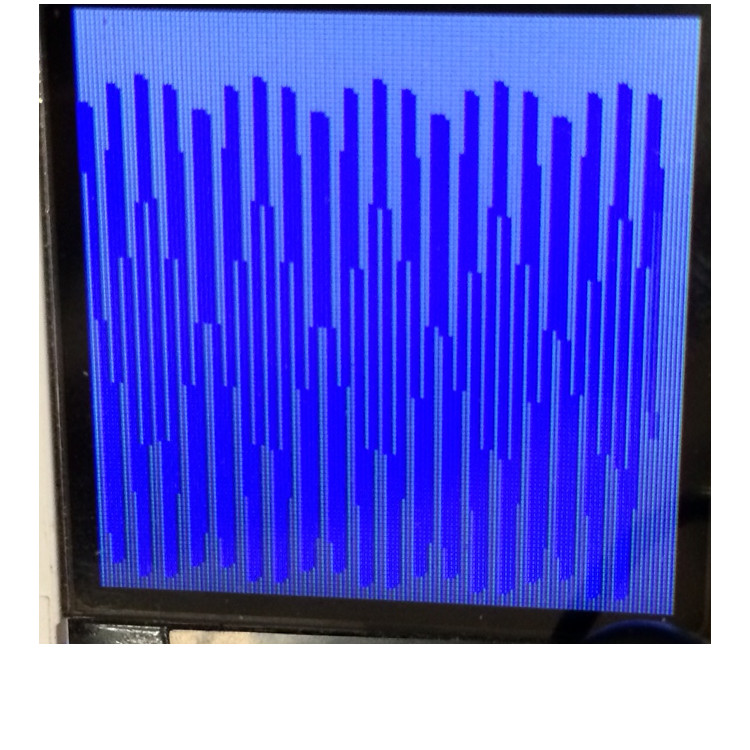
\includegraphics[width=0.375\textwidth]{./img/raw_500Hz}
      \caption{\texttt{Raw data 500 Hz plot}}
      \label{fig:raw_500}
    \end{figure}
  \end{paracol}
\item Digital scope data \\
  \begin{figure}[h!]
    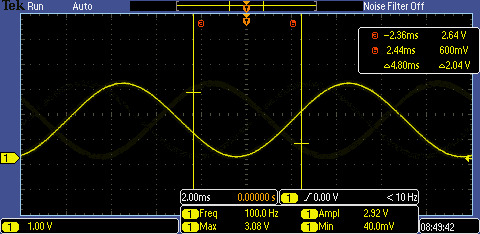
\includegraphics[width=0.375\textwidth]{./img/TEK00002}
    \caption{\texttt{Digital scope data: sampling 100 Hz}}
    \label{fig:dig_100}
  \end{figure}
  \begin{figure}[h!]
    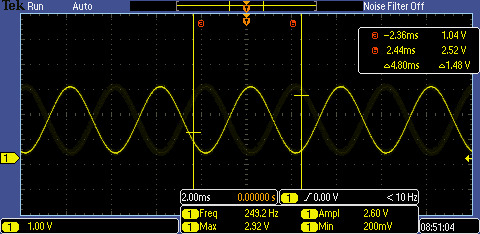
\includegraphics[width=0.375\textwidth]{./img/TEK00003}
    \caption{\texttt{Digital scope data: sampling 250 Hz}}
    \label{fig:dig_250}
  \end{figure}
  \begin{figure}[h!]
    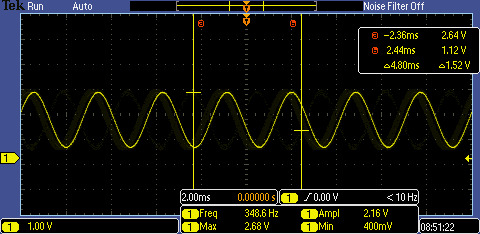
\includegraphics[width=0.375\textwidth]{./img/TEK00004}
    \caption{\texttt{Digital scope data: sampling 350 Hz}}
    \label{fig:dig_350}
  \end{figure}
  \begin{figure}[h!]
    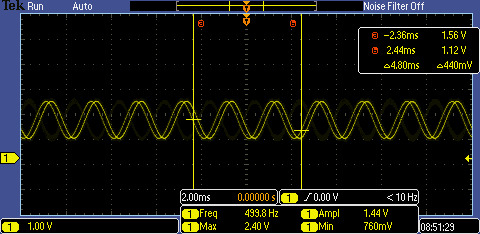
\includegraphics[width=0.375\textwidth]{./img/TEK00005}
    \caption{\texttt{Digital scope data: sampling 500 Hz}}
    \label{fig:dig_500}
  \end{figure}
  \begin{figure}[h!]
    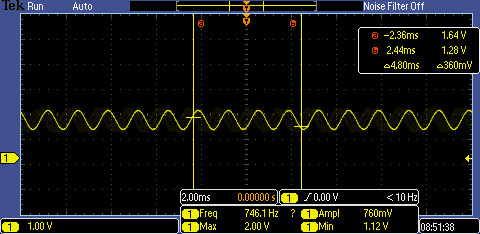
\includegraphics[width=0.375\textwidth]{./img/TEK00006}
    \caption{\texttt{Digital scope data: sampling 750 Hz}}
    \label{fig:dig_750}
  \end{figure}
  \begin{figure}[h!]
    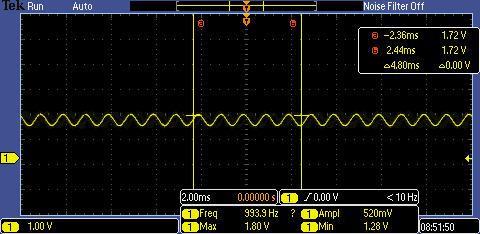
\includegraphics[width=0.375\textwidth]{./img/TEK00007}
    \caption{\texttt{Digital scope data: sampling 940 Hz}}
    \label{fig:dig_940}
  \end{figure}
  \begin{figure}[h!]
    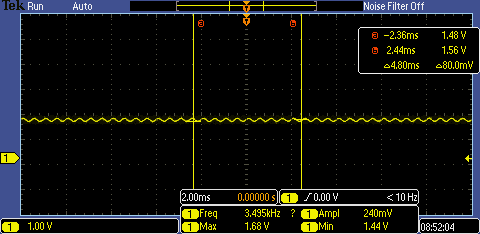
\includegraphics[width=0.375\textwidth]{./img/TEK00008}
    \caption{\texttt{Digital scope data: sampling 4 KHz}}
    \label{fig:dig_4000}
  \end{figure}
  \pagebreak % formatting gets worse without this -- you can probably
  % improve here
\item Spectrum analyzer data \\
  Absent
\item FIR filter test data \\
  Filtered and raw data are compared above. See references to the plots
  of filtered data (Figures \ref{fig:filtered_100} through \ref{fig:filtered_500}).
\end{enumerate}

\section{Analysis and Discussion}
\begin{enumerate}[1)]
\item How did measured frequency responses compare to your estimations
  of cutoff frequencies for your HPF and LPF? \\
  \todo The lowpass filter was created in Octave. TI's web bench tool
  calculated our analog LPF's cutoff frequencies.
\item Explain how you measured maximum bandwidth. What was the
  limiting factor affecting bandwidth? \\
  \todo since we don't have fft... isn't that going to be the most
  computationally intensive (bandwidth-limiting) section?
  \item What is the expected FFT output if the input is a square wave? \\
  Impulses on the harmonic frequencies of the square wave emerge on
  the frequency vs. apmlitude plot.
\item Look at the noise in your digital samples when it is very
  quiet. What noise is this? \\
  Error introduced by the sampling components, mathematical rounding
  errors and jitter. \todo verify
\item Can you estimate jitter in your ADC samples? \\
  No, we did not implement jitter calculation in this lab.
\item Prove your FIR implementation can not overflow. \\
\item Look at symmetry in the \verb|h[51]| coefficients in the example
  FIR design. How could you rewrite the following filter equation to
  reduce the number of multiplies from 51 to 26?
  $y[i]=(h[0]*x[i]+h[1]*x[i-1]+h[2]*x[i-2]+...+h[50]*x[i-50])/256;$ \\
  \todo I'm not sure... will revisit.
\item Explain how the multiple and accumulate instruction (MLA) can
  reduce the execution time of your filter. If you were to have used
  the MLA instruction, would your filter have been more accurate?

  MLA obviates the need for adding the products we determine to a
  separate accumulator. Since the accumulator is handled by MLA
  hardware, the amount of transferring bits around the
  microarchitecture at the speed of the bus clock is reduced. Similar
  to tail-chaining of interrupt service vectors, slight hardware
  optimization is provided for this common task.

  Our filter would have been more accurate since \verb|IEEE 754-2008|
  specifies this instruction must be implemented with only one
  rounding (instead of two). This reduces total error accumulation
  over time.
\end{enumerate}

\section{Code}
\lstinputlisting[language=C,label=lst:lab4,caption=\texttt{lab4.c}]{@doc-staging-area@/lab4.c}

\end{document}
